\documentclass[letterpaper,12pt]{article}

% --- PAQUETES DE IDIOMA
\usepackage[spanish,mexico]{babel}
\usepackage[utf8]{inputenc}
\usepackage{csquotes}

% --- PAQUETES MATEMÁTICOS --
\usepackage{amsmath}
\usepackage{amssymb}
\usepackage{cancel}
\usepackage{mathrsfs}

% --- PAQUETES GRÁFICOS Y DE DISEÑO ---
\usepackage{graphicx}
\usepackage{float}
\usepackage{subcaption}
\usepackage[table]{xcolor}
\usepackage{longtable}
\usepackage{multirow}
\usepackage{makecell}
\usepackage{array}
\usepackage{caption}
\usepackage{tikz}
\usetikzlibrary{decorations.pathmorphing}
\usepackage{circuitikz}
\usetikzlibrary{shapes.geometric, shapes.multipart, shapes.symbols, positioning, arrows.meta, calc, shadows, decorations.pathreplacing,babel}

% --- LISTAS ---
\usepackage{enumitem}

% --- PAQUETES DE CÓDIGO ---
\usepackage{listings}
% Configuración del estilo de listings
\definecolor{codebg}{rgb}{0.95,0.95,0.95}   
\definecolor{keyword}{rgb}{0.0,0.2,0.6}     
\definecolor{comment}{rgb}{0.25,0.5,0.35}   
\definecolor{string}{rgb}{0.6,0.0,0.0}      
\definecolor{number}{rgb}{0.5,0.0,0.5}      
\definecolor{codegray}{rgb}{0.5,0.5,0.5}
\definecolor{codepurple}{rgb}{0.58,0,0.82}
\definecolor{backcolour}{rgb}{0.95,0.95,0.95}

% Definición de los colores utilizados en las tablas
\definecolor{headerbg}{HTML}{5B84C4} % Azul oscuro para el encabezado principal
\definecolor{subheaderbg}{HTML}{B4C6E7} % Azul intermedio para sub-encabezados
\definecolor{rowbg}{HTML}{E9EDF4} % Azul claro para filas intercaladas

\lstset{
  backgroundcolor=\color{backcolour},
  basicstyle=\ttfamily\small,
    inputencoding=utf8,
  keywordstyle=\color{blue}\bfseries,
  stringstyle=\color{codepurple},
  commentstyle=\color{codegray}\itshape,
  numbers=left,
  numberstyle=\tiny\color{codegray},
  frame=single,
  rulecolor=\color{black},
  breaklines=true,
  tabsize=4,
  showstringspaces=false,
  literate={á}{{\'a}}1
           {é}{{\'e}}1
           {í}{{\'i}}1
           {ó}{{\'o}}1
           {ú}{{\'u}}1
           {Á}{{\'A}}1
           {É}{{\'E}}1
           {Í}{{\'I}}1
           {Ó}{{\'O}}1
           {Ú}{{\'U}}1
           {ñ}{{\~n}}1
           {Ñ}{{\~N}}1
           {¿}{{\textquestiondown}}1
           {¡}{{\textexclamdown}}1
           {°}{{\ensuremath{^\circ}}}1
}

% Definición del lenguaje Python para listings
\lstdefinelanguage[LAB]{Python}{
    morekeywords={False, None, True, and, as, assert, async, await, break,
                                class, continue, def, del, elif, else, except, finally,
                                for, from, global, if, import, in, is, lambda, nonlocal,
                                not, or, pass, raise, return, try, while, with, yield,
                                machine, Pin, PWM, ADC, Timer, sleep_ms, sleep_us},
    morecomment=[l]{\#},
    morestring=[b]",
    morestring=[b]',
    sensitive=true
}

% --- ESTILOS PARA DIAGRAMAS DE FLUJO (TIKZ) ---
\tikzset{
  startstop/.style={rectangle, rounded corners, minimum width=3cm, minimum height=1cm,text centered, draw=black, fill=red!30},
  process/.style={rectangle, minimum width=3cm, minimum height=1cm, text centered, draw=black, fill=orange!30},
  decision/.style={diamond, aspect=2, minimum width=3cm, minimum height=1cm, text centered, draw=black, fill=green!30},
  io/.style={trapezium, trapezium left angle=70, trapezium right angle=110, minimum width=3cm, minimum height=1cm, text centered, draw=black, fill=blue!30},
  arrow/.style={thick,->,>=stealth}
}

% Definimos el color dorado/naranja para el cuadro de texto
\definecolor{goldbox}{RGB}{218, 140, 15}

% Macro para dibujar la Raspberry Pi Pico y sus nodos
\newcommand{\picoboard}{
    \draw[thick] (0,0.5) rectangle (4,-9.5);
    \node[align=center, font=\small\sffamily] at (2, -1.5) {Raspberry PI\\[0.1cm]Pico};

    % Pines Superiores
    \draw[red, thick] (0.8, 0.5) -- (0.8, 0.8) coordinate (P41); \node[above, font=\tiny\sffamily, inner sep=1pt] at (P41) {41};
    \draw[red, thick] (2.0, 0.5) -- (2.0, 0.8) coordinate (P42); \node[above, font=\tiny\sffamily, inner sep=1pt] at (P42) {42};
    \draw[red, thick] (3.2, 0.5) -- (3.2, 0.8) coordinate (P43); \node[above, font=\tiny\sffamily, inner sep=1pt] at (P43) {43};
    \node[below, font=\tiny\sffamily] at (0.8, 0.5) {SW CLK};
    \node[below, font=\tiny\sffamily] at (2.0, 0.5) {SW GND};
    \node[below, font=\tiny\sffamily] at (3.2, 0.5) {SW DIO};

    % GND Inferior
    \draw[red, thick] (2, -9.5) -- (2, -10.2) coordinate (PGND);
    \node[above, font=\tiny\sffamily] at (2, -9.5) {GND};
    \node[below, font=\tiny\sffamily] at (2, -10.2) {3,8,13,18 \quad 23,28,38};

    % Pines del lado Izquierdo
    \foreach \i/\pin/\num in {
        1/GP0/1, 2/GP1/2, 
        4/GP2/4, 5/GP3/5, 6/GP4/6, 7/GP5/7, 
        9/GP6/9, 10/GP7/10, 11/GP8/11, 12/GP9/12, 
        14/GP10/14, 15/GP11/15, 16/GP12/16, 17/GP13/17, 
        19/GP14/19, 20/GP15/20
    } {
        \draw[red, thick] (0, -\i*0.45) -- (-0.4, -\i*0.45) coordinate (P\num);
        \node[right, font=\tiny\sffamily] at (0, -\i*0.45) {\pin};
        \node[above left, font=\tiny\sffamily, inner sep=1pt] at (P\num) {\num};
    }

    % Pines del lado Derecho
    \foreach \i/\pin/\num in {
        1/VBUS/40, 2/VSS/39, 
        4/3V3\_EN/37, 5/3V3/36, 6/ADC\_VREF/35, 7/GP28\_A2/34, 8/AGND/33, 
        9/GP27\_A1/32, 10/GP26\_A0/31, 11/RUN/30, 12/GP22/29, 
        14/GP21/27, 15/GP20/26, 16/GP19/25, 17/GP18/24, 
        19/GP17/22, 20/GP16/21
    } {
        \draw[red, thick] (4, -\i*0.45) -- (4.4, -\i*0.45) coordinate (P\num);
        \node[left, font=\tiny\sffamily] at (4, -\i*0.45) {\pin};
        \node[above right, font=\tiny\sffamily, inner sep=1pt] at (P\num) {\num};
    }
}



\definecolor{azulresultado}{HTML}{0072C6}
\definecolor{rojoacarreo}{HTML}{FF0000}

% Colores para la tabla
\definecolor{headblue}{HTML}{4F81BD}
\definecolor{subheadblue}{HTML}{B8CCE4}
\definecolor{datablockblue}{HTML}{DCE6F1}

% --- RUTAS DE IMÁGENES ---
\graphicspath{{img/}{portada_img/}}

\definecolor{armblue}{RGB}{0, 113, 188}

% --- CONFIGURACIÓN DE PÁGINA (GEOMETRÍA) ---
\usepackage[
    left=25mm, 
    right=25mm,
    top=35mm,
    bottom=30mm,
    headheight=77pt, 
    papersize={21.59cm,27.94cm}
]{geometry}

% --- FORMATO DE TEXTO ---
\renewcommand{\baselinestretch}{1.25} 
\usepackage{parskip} 
\usepackage{lipsum}  

% --- VARIABLES GLOBALES ---
\newcommand{\materia}{}

% --- ENCABEZADOS Y PIES DE PÁGINA ---
\usepackage{fancyhdr}
\pagestyle{fancy}
\fancyhf{} 
\fancyhead[L]{
\includegraphics[height=1.5cm]{portada_img/izq.png}}
\fancyhead[R]{
\includegraphics[height=1.5cm]{portada_img/der.png}}
\fancyfoot[C]{\thepage} 
\renewcommand{\headrulewidth}{0.4pt} 
\renewcommand{\footrulewidth}{0pt}  

% --- BIBLIOGRAFÍA ---
\usepackage[backend=biber, style=apa, sortcites, url=true]{biblatex}
\addbibresource{referencias.bib}

% --- HIPERVÍNCULOS ---
\usepackage{hyperref}
\hypersetup{
    colorlinks=true,
    linkcolor=blue,
    citecolor=blue,
    filecolor=magenta,
    urlcolor=cyan
}

\begin{document}

    \input{portada.tex}

    \newpage
    \setcounter{page}{1}

    \section{Objetivo:}
    
    Aprender el funcionamiento de la comunicación serial en la modalidad asíncrona para la
    transferencia de información entre diferentes dispositivos por medios alámbricos e inalámbricos.

    \section*{Actividad 1}
    Escribir el siguiente programa:
    \lstinputlisting[language={[LAB]Python}, caption=Código de ejemplo; actividad 1, basicstyle=\ttfamily\scriptsize]{Code/Act1Normal.py}
    \begin{enumerate}
        \item Comentar el código.
        \item Indicar que hace: 
        El programa implementa un sistema de lectura de datos a través del puerto serie de manera asíncrona o no bloqueante. Inicialmente, configura un objeto de sondeo (\textit{polling}) para monitorear el flujo de entrada estándar (\texttt{sys.stdin}). Durante su ciclo de ejecución infinito, el microcontrolador verifica continuamente si el usuario ha tecleado un dato en la consola sin detener el hilo principal de procesamiento. En el momento en que detecta información en el búfer de entrada, extrae exactamente un carácter y responde enviando cadenas de texto predefinidas ("Dato recibido" y "Hola UNAM") hacia el monitor serial, finalizando la iteración con un retardo de 100 milisegundos para no saturar los recursos de la CPU.
        
        \item Ejecutar
        \item Ingresar datos desde la consola de Thonny.
        \item Explicar la diferencia entre:
        \begin{itemize}
            \item \textbf{\texttt{sys.stdout.write()}:} Es una función de bajo nivel que interactúa directamente con el flujo de salida estándar del sistema  . Escribe la cadena de texto de forma estricta, sin agregar ningún formato adicional. Por esta razón, el programador debe incluir explícitamente el salto de línea (\texttt{$\backslash$n}) al final de la cadena si desea pasar al siguiente renglón.
            \item \textbf{\texttt{print()}:} Es una función de alto nivel en Python que internamente utiliza \texttt{sys.stdout.write()}, pero funciona como una envoltura (\textit{wrapper}) que procesa los datos  . Automáticamente inserta espacios entre múltiples argumentos y, por defecto, agrega un salto de línea al final de la impresión, facilitando la lectura humana en la consola.
        \end{itemize}
    \end{enumerate}

    \subsection*{Propuesta de solución}
    El objetivo del código es implementar un sistema de lectura de datos a través del puerto serie (USB) de manera no bloqueante. Tradicionalmente, funciones como \texttt{input()} detienen por completo la ejecución del procesador hasta que el usuario ingresa un dato. Para evitar esto, se propone el uso del módulo \texttt{select}, el cual permite sondear (\textit{polling}) el búfer de entrada estándar (\texttt{sys.stdin})  . El programa registra este flujo de entrada y, mediante un ciclo infinito, verifica si hay algún byte esperando ser leído en el búfer sin detener el procesador  . Si se detecta información, se extrae exactamente un carácter y se imprime un mensaje de confirmación  .

     El flujo de datos de este código inicia con la importación de las bibliotecas necesarias para monitorear el flujo de entrada en la consola. Se registra la entrada estándar y se manda a imprimir un mensaje indicando que se está esperando un carácter. Posteriormente, el programa entra en un bucle infinito que constantemente comprueba la función \texttt{poll(0)}. Si llega alguna información desde Thonny al microcontrolador a través del USB, el condicional se activa, lee exactamente un dato e imprime inmediatamente un respectivo "Hola UNAM". Independientemente de si detecta datos o no, se realiza una pausa de 100 milisegundos al final de cada iteración para que el procesador no se sature.

    \begin{figure}[H]
            \centering
            \begin{tikzpicture}[node distance=1.5cm, every node/.style={scale=0.8}]
                \node (start) [startstop] {Inicio};
                \node (import) [process, below of=start] {Importar módulos};
                \node (init) [process, below of=import] {Inicializar \texttt{poll\_obj}};
                \node (reg) [process, below of=init] {Registrar \texttt{sys.stdin}};
                \node (print) [io, below of=reg, align=center] {Mostrar mensajes\\iniciales};
                \node (loop) [decision, below of=print, yshift=-0.8cm] {¿\texttt{poll(0)} es True?};
                
                % 1. Aumentamos el xshift a 4cm para separar la caja del rombo
                \node (read) [process, right of=loop, xshift=4cm] {Leer carácter (\texttt{ch})};
                
                \node (print2) [io, below of=read, yshift=-0.5cm, align=center] {Imprimir \texttt{'Dato recibido'}\\y \texttt{'Hola UNAM'}};
                
                % 2. Bajamos un poco más la pausa (yshift=-2.5cm) para que la flecha de print2 no quede apretada
                \node (delay) [process, below of=loop, yshift=-2.5cm] {Pausa (\texttt{time.sleep(0.1)})};
                
                \draw [arrow] (start) -- (import);
                \draw [arrow] (import) -- (init);
                \draw [arrow] (init) -- (reg);
                \draw [arrow] (reg) -- (print);
                \draw [arrow] (print) -- (loop);
                
                % 3. Ajustamos la posición del texto "Sí" (pos=0.4) y lo levantamos un poquito (yshift=0.05cm)
                \draw [arrow] (loop) -- node[anchor=south, pos=0.4, yshift=0.05cm] {Sí} (read);
                
                \draw [arrow] (read) -- (print2);
                \draw [arrow] (print2) |- (delay);
                \draw [arrow] (loop) -- node[anchor=east] {No} (delay);
                \draw [arrow] (delay.south) -- ++(0,-0.5) -| +(-3,0) |- (loop.west);
            \end{tikzpicture}
            \caption{Diagrama de flujo representativo de la Actividad 1}
            \label{fig:flujo_act1}
    \end{figure}

    \subsection*{Desarrollo}

    \lstinputlisting[language={[LAB]Python}, caption=Código de la Actividad 1, basicstyle=\ttfamily\scriptsize]{Code/Act1.py}

    \begin{figure}[H]
        \centering
        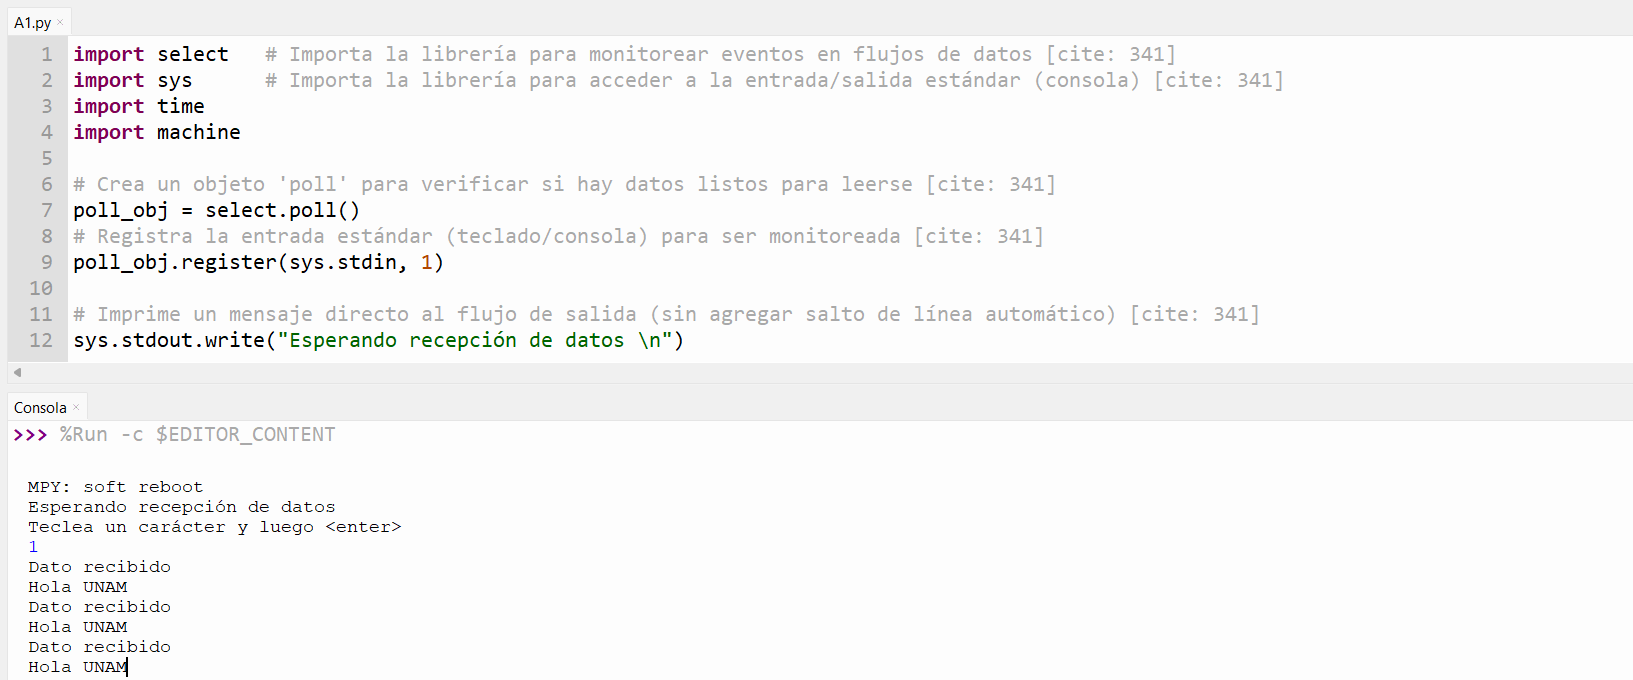
\includegraphics[width=0.85\textwidth]{ img/Actividad1/Act1_1.png}
        \caption{Interacción asíncrona a través de la terminal serial. La consola muestra los mensajes de inicialización solicitando la entrada del usuario. Al teclear un carácter, el objeto \texttt{poll} detecta de forma instantánea la actividad en el búfer de entrada (\texttt{sys.stdin}). El microcontrolador extrae el dato y ejecuta las instrucciones de impresión ("Dato recibido" y "Hola UNAM"), demostrando la lectura exitosa sin detener el flujo continuo del procesador.}
    \end{figure}

    \subsection*{Análisis de resultados}
    Al ejecutar el programa en Thonny, pudimos comprobar que la recepción de datos de manera asíncrona funciona correctamente. Mientras el usuario no presione ninguna tecla o envíe parámetros, la instrucción \texttt{poll\_obj.poll(0)} le dice al procesador principal que, al no haber datos en el puerto, puede realizar su pausa de 0.1 s y seguir dando vueltas en lugar de quedarse trabado esperando. En el momento en que enviamos desde la consola un carácter y presionamos Enter, el carácter viaja a la memoria desde la computadora usando el puerto serie y en el siguiente ciclo será detectado; en ese momento el sistema lee y vacía un byte del \textit{buffer} para finalmente dar la señal de mostrar los mensajes confirmatorios. Gracias a esto comprobamos el beneficio del ``no-bloqueo".

    \newpage

    \newpage

    \section*{Actividad 2}
    Para este ejercicio, realizar los pasos siguientes:
    \begin{enumerate}
        \item Ubicar el COM de conexión de la Raspberry Pi.
        \item Abrir la terminal de su preferencia.
        \item Explicar si existe alguna diferencia en la ejecución y cuál sería el motivo.
    \end{enumerate}
        
    \subsection*{Propuesta de solución}


    \subsection*{Desarrollo}


    \subsection*{Análisis de resultados}
    

    \newpage
    \section*{Actividad 3}
    Utilizando el formato de la actividad 1, realizar un programa que reciba comandos a través del puerto serie y ejecute las acciones indicadas.

    \begin{table}[h]
        \centering
        \begin{tabular}{|c|c|}
        \hline
        \rowcolor[HTML]{5B9BD5} 
        \textcolor{white}{\textbf{Dato recibido}} & \textcolor{white}{\textbf{Acción}} \\ \hline
        `0' & GPIO25 = OFF \\ \hline
        `1' & GPIO25 = ON \\ \hline
        \end{tabular}
        \caption*{Tabla 7-2. Control; actividad 3}
    \end{table}

    \vspace{0.5cm}

    \subsection*{Propuesta de solución}
    Esta actividad combina la lectura no bloqueante del puerto serie con el control directo de las salidas digitales del microcontrolador . Se configura el pin físico \texttt{GPIO25} (conectado al LED integrado de la Raspberry Pi Pico) como una salida digital (\texttt{Pin.OUT}) . Replicando la estructura de sondeo con el módulo \texttt{select}, el programa extrae los caracteres entrantes desde la consola de Thonny .

    El control se realiza mediante una estructura condicional \texttt{if-elif} . El carácter recuperado por \texttt{sys.stdin.read(1)} se compara contra los caracteres ASCII de control definidos en la tabla . Si el programa recibe el carácter \texttt{'1'}, saturará el pin a nivel alto ; si recibe \texttt{'0'}, drenará el voltaje a nivel bajo . Cualquier otro carácter (como letras o el retorno de carro enviado al presionar Enter) será simplemente ignorado por el flujo condicional, evitando falsas activaciones.

    \begin{figure}[H]
            \centering
            \begin{tikzpicture}[node distance=1.5cm, every node/.style={scale=0.75}]
                \node (start) [startstop] {Inicio};
                \node (init) [process, below of=start] {Configurar LED y \texttt{poll\_obj}};
                \node (reg) [process, below of=init] {Registrar \texttt{sys.stdin}};
                \node (print) [io, below of=reg, align=center] {Mostrar instrucciones};
                \node (loop) [decision, below of=print, yshift=-0.5cm] {¿\texttt{poll(0)} es True?};
                \node (read) [process, right of=loop, xshift=4cm] {Leer (\texttt{ch = read(1)})};
                \node (cond1) [decision, below of=read, yshift=-1.5cm] {¿\texttt{ch} == '1'?};
                
                % 1. Aumentamos el xshift a 3.8cm para alargar más la flecha
                \node (ledOn) [process, right of=cond1, xshift=3.8cm, align=center] {Encender LED y print};
                
                \node (cond2) [decision, below of=cond1, yshift=-1.5cm] {¿\texttt{ch} == '0'?};
                
                % 1. Aumentamos el xshift a 3.8cm también aquí
                \node (ledOff) [process, right of=cond2, xshift=3.8cm, align=center] {Apagar LED y print};
                
                \node (delay) [process, below of=loop, yshift=-7.5cm] {Pausa (\texttt{time.sleep(0.1)})};
                
                \draw [arrow] (start) -- (init);
                \draw [arrow] (init) -- (reg);
                \draw [arrow] (reg) -- (print);
                \draw [arrow] (print) -- (loop);
                \draw [arrow] (loop) -- node[anchor=south] {Sí} (read);
                \draw [arrow] (read) -- (cond1);
                
                % 2. Añadimos pos=0.4 para acercar el "Sí" al rombo y yshift=0.05cm para despegarlo de la línea
                \draw [arrow] (cond1) -- node[anchor=south, pos=0.4, yshift=0.05cm] {Sí} (ledOn);
                \draw [arrow] (cond1) -- node[anchor=east] {No} (cond2);
                
                % 2. Mismo ajuste para esta flecha
                \draw [arrow] (cond2) -- node[anchor=south, pos=0.4, yshift=0.05cm] {Sí} (ledOff);
                
                \draw [arrow] (loop) -- node[anchor=east] {No} (delay);
                \draw [arrow] (ledOn) |- (delay);
                \draw [arrow] (ledOff) |- (delay);
                \draw [arrow] (cond2) |- node[anchor=east, pos=0.15] {No} (delay);
                \draw [arrow] (delay.south) -- ++(0,-0.5) -| +(-3.8,0) |- (loop.west);
            \end{tikzpicture}
            \caption{Diagrama de flujo de la Acción 3}
            \label{fig:flujo_act3}
    \end{figure}

    Este flujo inicializa estableciendo el pin del LED (25) como salida, configurando al igual el objeto para leer el teclado con \texttt{select.poll()}, y luego, notifica al usuario qué presionar dentro del panel interactivo de Thonny. Para evitar bloqueos, un ciclo eterno va sondeando si se recibe algún byte mediante  el condicional del objeto \texttt{poll}. De ser afirmativo, almacena la cadena; entra al subproceso de comprobación anidados por medio de \texttt{if} y compara, si tecleó '1' pasará voltaje positivo, y si la coincidencia fue '0' apaga dicho Pin. Tras efectuar las comprobaciones de los posibles escenarios o de no haberse escrito absolutamente nada en consola, detiene por 0.1 segundos el procedimiento de barrido principal y todo vuelve a empezar.

    \subsection*{Desarrollo}

    \lstinputlisting[language={[LAB]Python}, caption=Código de la Actividad 3, basicstyle=\ttfamily\scriptsize]{Code/Act3.py}

    \begin{figure}[H]
        \centering
        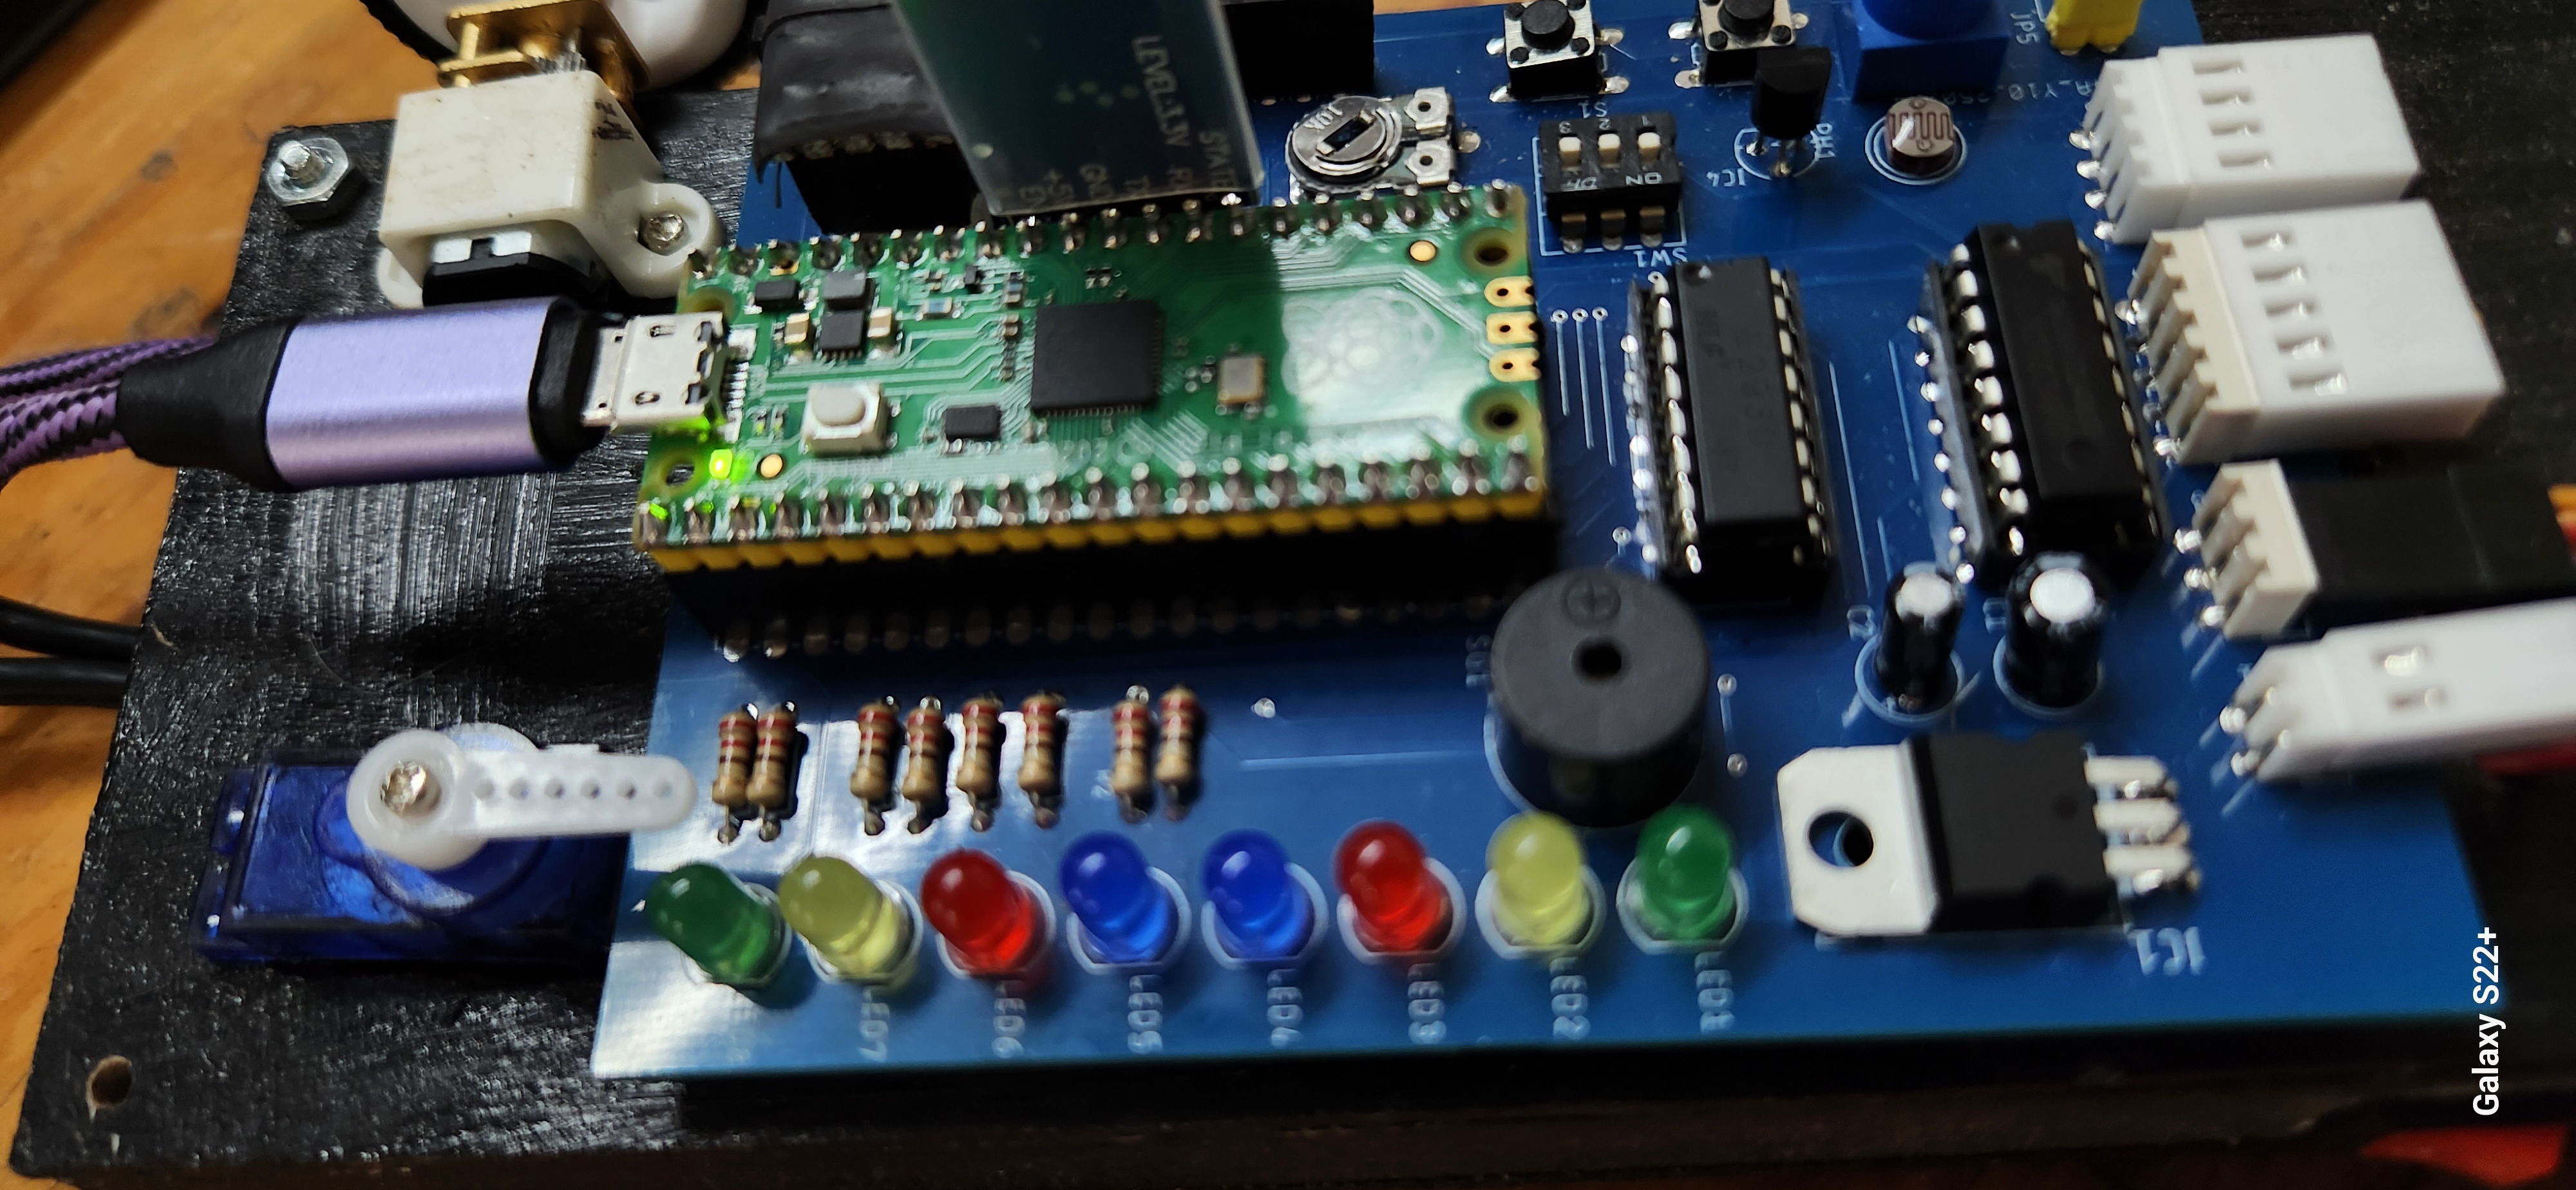
\includegraphics[width=0.7\textwidth]{ img/Actividad3/Act3_1.jpg}
        \caption{Activación del actuador interno. El usuario ingresa el carácter '1' a través de la terminal USB. El microcontrolador RP2040 intercepta el dato mediante el sondeo del búfer, evaluando la primera condicional como verdadera. Inmediatamente, satura el pin físico GPIO 25, encendiendo el LED verde integrado en la tarjeta y confirmando la acción en consola.}
    \end{figure}

    \begin{figure}[H]
        \centering
        
\includegraphics[width=0.7\textwidth]{ img/Actividad3/Act3_2.jpg}
        \caption{Desactivación mediante consola. Al teclear el carácter '0', el sistema captura el nuevo evento de entrada. La rutina de control procesa el carácter ASCII, el flujo salta a la segunda rama condicional y el hardware drena el voltaje del GPIO 25 (0V). Esto apaga el LED físico y envía la confirmación de la acción completada al monitor serial.}
    \end{figure}
    
    \begin{figure}[H]
        \centering
        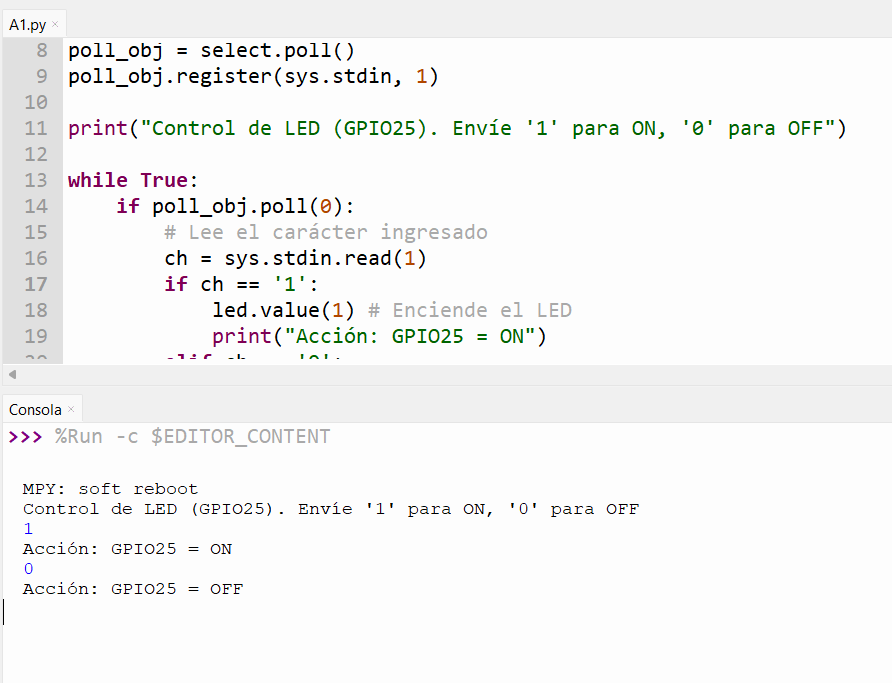
\includegraphics[width=0.6\textwidth]{ img/Actividad3/Act3_3.png}
        \caption{Monitor serial Thonny. Captura de pantalla evidenciando la bitácora bidireccional (\textit{log}) de la comunicación asíncrona entre el entorno de desarrollo y el hardware embebido.}
    \end{figure}

    \subsection*{Análisis de resultados}
    Este ejercicio ilustra de manera muy visual cómo lograr una interacción en tiempo real de control mediante un bucle cerrado; entre la computadora principal desde la que mandamos instrucciones y el \textit{hardware} esclavo que las recibe. Cuando corremos este código, observamos que luego de un simple mensaje se mantiene monitoreando pacientemente el monitor y dejando libre el micro. Si le escribimos un '1', la tarjeta responde físicamente alimentando el encendido del LED conectado al GPIO 25, con su debida contestación en la interfaz de "GPIO25 = ON". Algo análogo sucede si enviamos un '0', se drenaría hacia masa apagándose visiblemente al instante. Demostrando cómo el manejo de comandos básicos sobre comunicación UART y lectura asíncrona construyen programas más estables en cualquier sistema electrónico empotrado contemporáneo de bajo coste sin importar las pausas del usuario.
    
    \newpage
    \section*{Actividad 4}
    Realizar el siguiente procedimiento:

    \begin{enumerate}
        \item Escribir el siguiente programa.
        \item Comentar el código e indicar que hace
        \item Conectar el módulo CP2102.
        \item Ubicar el puerto asignado.
        \item Comprobar el funcionamiento
    \end{enumerate}

    \lstinputlisting[language={[LAB]Python}, caption=Código de ejemplo; actividad 4, basicstyle=\ttfamily\scriptsize]{Code/Act4Normal.py}




    \subsection*{Propuesta de solución}



    \subsection*{Desarrollo}

    \lstinputlisting[language={[LAB]Python}, caption=Código de la Actividad 4, basicstyle=\ttfamily\scriptsize]{Code/Act4.py}



    \subsection*{Análisis de resultados}


    \newpage

    \section*{Actividad 5}

    Siguiendo el procedimiento de la actividad No. 4; realizar un programa que ejecute las acciones indicadas.

    \begin{table}[h]
        \centering
        \begin{tabular}{|c|l|}
            \hline
            \rowcolor[HTML]{5B9BD5} 
            \textcolor{white}{\textbf{\shortstack{Dato \\ UART}}} & \multicolumn{1}{c|}{\cellcolor[HTML]{5B9BD5}\textcolor{white}{\textbf{Acción}}} \\ \hline
            `1' & Mostrar el voltaje del Potenciómetro \\ \hline
            `2' & Mostrar el resultado de la conversión AD de la foto-resistencia en hexadecimal. \\ \hline
            `3' & Mostrar la temperatura del sensor TMP36 en $^{\circ}$C, $^{\circ}$F y $^{\circ}$K. \\ \hline
            `4' & Reproducir la nota DO en el zumbador \\ \hline
            `5' & Prender y apagar 5 veces GPIO0 al GPIO7 \\ \hline
            `6' & Corrimiento a la derecha de los 8 leds GPIO0 -- GPIO7 \\ \hline
            `7' & Corrimiento a la izquierda de los 8 leds GPIO0 -- GPIO7 \\ \hline
        \end{tabular}
        \caption*{Tabla 7-3. Tabla de control; actividad 5}
    \end{table}

    \vspace{0.5cm}


    \subsection*{Propuesta de solución}


    \subsection*{Desarrollo}

    \lstinputlisting[language={[LAB]Python}, caption=Código de la Actividad 5 Comentado,basicstyle=\ttfamily\scriptsize]{Code/Act5.py}



    \subsection*{Análisis de resultados}


    \newpage

    \section*{Actividad 6}
    Conectando el módulo bluetooth, realizar un programa que ejecute las acciones indicadas en la tabla 7-4.

    \begin{table}[h]
        \centering
        \begin{tabular}{|c|c|}
            \hline
            \rowcolor[HTML]{5B9BD5} 
            \textcolor{white}{\textbf{Dato recibido}} & \textcolor{white}{\textbf{Acción}} \\ \hline
            `A' & GPIO0 = ON \\ \hline
            `T' & GPIO1 = ON \\ \hline
            `D' & GPIO2 =ON \\ \hline
            `I' & GPIO3 =ON \\ \hline
            S & GPIO0:GPIO3 = OFF \\ \hline
        \end{tabular}
        \caption*{Tabla 7-4. Control; actividad 6}
    \end{table}

    \noindent \textit{\textcolor[HTML]{4A72B8}{Nota: Descargar la aplicación de control bluetooth de la página del Laboratorio de Microcomputadoras.}}

    \vspace{0.5cm}


    \subsection*{Propuesta de solución}


    \subsection*{Desarrollo}

    \lstinputlisting[language={[LAB]Python}, caption=Código de la Actividad 6,basicstyle=\ttfamily\scriptsize]{Code/Act6.py}

    \subsection*{Análisis de resultados}


    \newpage
    \section*{Actividad 7}
    Realizar un programa que controle el funcionamiento de los motores de Corriente Directa de la practica 5, por medio de la comunicación serie empleando el módulo Bluetooth.

    \begin{table}[h]
        \centering
        \begin{tabular}{|c|c|c|}
            \hline
            \rowcolor[HTML]{5B9BD5} 
            \cellcolor[HTML]{5B9BD5}\textcolor{white}{\textbf{Comando}} & \multicolumn{2}{c|}{\cellcolor[HTML]{5B9BD5}\textcolor{white}{\textbf{ACCION}}} \\ \cline{2-3} 
            \rowcolor[HTML]{5B9BD5} 
            \cellcolor[HTML]{5B9BD5}\textcolor{white}{\textbf{Puerto Serie}} & \cellcolor[HTML]{D9E2F3}\textbf{MOTOR 1} & \cellcolor[HTML]{D9E2F3}\textbf{MOTOR 2} \\ \hline
            ``S'' & PARO & PARO \\ \hline
            ``A'' & HORARIO & HORARIO \\ \hline
            ``T'' & ANTI-HORARIO & ANTI-HORARIO \\ \hline
            ``D'' & HORARIO & ANTI-HORARIO \\ \hline
            ``I'' & ANTI-HORARIO & HORARIO \\ \hline
        \end{tabular}
        \caption*{Tabla 7-5. Control UART; actividad 7}
    \end{table}

\noindent \textit{\textcolor[HTML]{4A72B8}{Nota: Descargar la aplicación de control bluetooth de la página del Laboratorio de Microcomputadoras.}}



    \section*{Propuesta de solución}



    \section*{Desarrollo}

    \lstinputlisting[language={[LAB]Python}, caption=Código de la Actividad 7,basicstyle=\ttfamily\scriptsize]{Code/Act7.py}

    \subsection*{Análisis de resultados}


    \newpage
    \section{Conclusiones:}

    \begin{itemize}
        \item \textbf{Espinoza Matamoros Percival Ulises:} 

        \item \textbf{Flores Colin Victor Jaziel:}

        \item \textbf{Lara Hernandez Angel Husiel:} En esta práctica comprendí la importancia y el funcionamiento de la comunicación serial asíncrona, enfocándome en el uso del módulo \texttt{select} para evitar bloqueos en el microcontrolador. Al utilizar funciones como \texttt{poll(0)} y \texttt{read(1)}, noté cómo el procesador puede seguir ejecutando otras tareas de fondo mientras está a la espera de recibir instrucciones, lo que es un enfoque muchísimo más eficiente que detener todo el flujo del programa esperando que el usuario ingrese un comando.
        
        Implementar este envío y recepción de  datos para desencadenar acciones físicas, como encender un LED o configurar el giro y paro de motores de corriente directa con un módulo Bluetooth, me sirvió mucho para ver la aplicación práctica de estos conceptos. 

    \end{itemize}

    \newpage

    % Impresión Referencias
    \nocite{*}
    \printbibliography[heading=bibintoc, title={Referencias}]
\end{document}